%------------------------------------------------------------------------
% Chapter:  1D data plots
%------------------------------------------------------------------------

\chapter{Plotting 1D data \label {1d}}

In this chapter we will learn how to read, plot and print simple
1D data sets, e.g.  xy-data.  Chapter \ref{2d} explains the
plotting of 2D data sets.  However, many of the commands to modify
a plot discussed in this chapter also apply to the plotting of 2D
data.

\begin{figure}[!b]
   \centering
   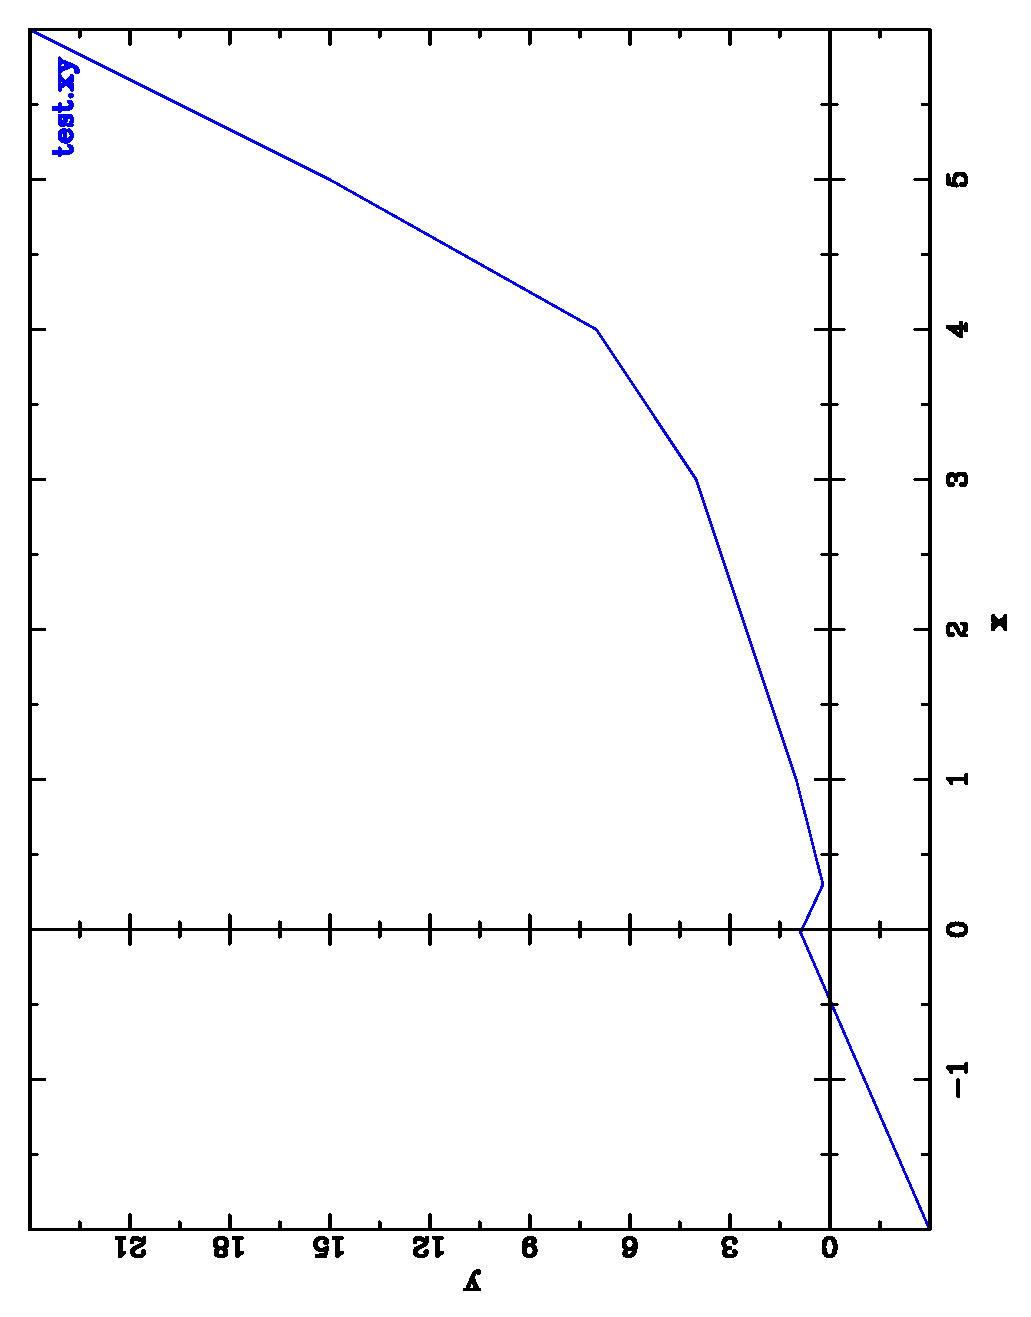
\includegraphics[width=3.0in, angle=270.0]{pl1.1.eps}
   \caption{The first {\it KUPLOT} plot}
   \label{pl1-fig1}
\end{figure}

The simplest data file is a text file with x- and y-coordinates
($x_{i},y_{i}$) for each point in a separate line, as in the example
data file {\it test.xy} listed below:
%
\begin{MacVerbatim}
    -2.00 -3.00
    -0.02  0.87
      :     :
\end{MacVerbatim}
%
In order to plot the file {\it test.xy}, we only need to enter the
following two commands at the {\it KUPLOT} input prompt:
%
\begin{MacVerbatim}
    load xy,test.xy
    plot
\end{MacVerbatim}
%
The {\tt load} command reads the specified data file, which is in
our case of the type 'xy'. The command {\tt plot} finally displays
the plot on the screen. The resulting plot for this example can be
seen in Figure \ref{pl1-fig1}. The following sections of this
chapter describe the supported file formats and how to change, print
and save the resulting plots.

%------------------------------------------------------------------------

\section{File formats \label{1d-read}}

{\it KUPLOT} reads data sets using the 'load' command.  The simplest
file format is a text file containing values for $x$ and $y$ on a
separate line for each data point as in the previous example.  To
read more than one data set just repeat the {\tt load} command.  The
maximum number of data sets that can be read and the maximum total
number of data points are defined in the file {\it kuplot.inc} and
might be adjusted before {\it KUPLOT} is compiled. The current
limits can be displayed using the command {\tt show config}. The
{\tt rese} command clears the currently loaded data sets and the
next file is read as data set one again. \par

The various file formats for 1D data supported by {\it KUPLOT} are
summarized in Table \ref{pl1-tab1}. The file format is specified as
first parameter for the {\tt load} command followed by the name of
the file to be read. Note that the 'xy' and 'yx' formats may contain
standard deviations $\sigma_{x}, \sigma_{y}$ for each data point
which may be used to plot error bars using the {\tt etyp} command in
{\it KUPLOT}. Optional parameters for the command {\tt load xy}
allow one to assign columns in the data file to $x, y$ and
$\sigma_{x}, \sigma_{y}$. The following command for example will
assign column 2 to $x$, column 4 to $y$ and column 9 to $\sigma_{x}$
and 12 to $\sigma_{y}$:
%
\begin{MacVerbatim}
    load xy,datafile.dat,2,4,9,12
\end{MacVerbatim}
\par

\begin{table}[!bt]
\centering
\begin{tabularx}{\textwidth}{|p{15mm}|X|}
  \hline
  {\bf Format} & {\bf Description} \\
  \hline\hline
  cr   & Special crystal structure format exported by {\it DISCUS}.
         Each line contains $x$,$y$,$z$, marker type, color and
         marker size for the atom at the given coordinates. Note,
         the first two columns are uses for plotting, the $z$ value
         is ignored (see {\it DISCUS} plot sublevel). \\
  ma   & Only the $x$ value of each data line is read, $y$ is set to
         zero. This allows the plotting of tick marks (e.g. at Bragg peak
         positions) at the x-axis. \\
  sc/st & This command allows one to read scans from a SPEC file.\\
  gs   & This command allows one to read GSAS files.\\
  xx   & Each line contains only one value that is taken as $y$
         value and the point number is stored as $x$ value. \\
  xy   & Each line of the data file contains $x$,$y$ and optionally
         standard deviations $\sigma_{x}$ and $\sigma_{y}$ from a
         multi-column text file. The default is $x,y,\sigma_x,\sigma_y$,
         but the columns can also me manually assigned (see example).\\

  \hline
  special & Various other file formats are available to read specific
            information from data files created by the diffractometer
            control software for the instruments MAN I and MAN II at
            the FRM I.  For details refer to the online help for the
            command {\tt load}.\\
  \hline
\end{tabularx}
\caption{\label{pl1-tab1}Supported file formats for 1D data}
\end{table}

After a data set is read, {\it KUPLOT} displays the number of points
read and the x- and y-limits. In our previous example, the screen
output after entering the {\tt load xy,test.xy} looks like that:
%
\begin{MacVerbatim}
    Reading 2 columns ...
    Data set no.:   1

      Filename : test.xy                            (     8 points )
      Range  x :   -2.000     to    6.000
      Range  y :   -3.000     to    24.00
\end{MacVerbatim}
%
Since our example file contains no $\sigma$ values, {\it KUPLOT} can
only read two columns. The file is associated with data set 1. This
data set number is subsequently used to alter the appearance of the
plot for a given data set (see section \ref{1d-change}).

\subsection*{Reading SPEC files}

As mentioned earlier, {\it KUPLOT} can read so called SPEC files.
Basically a SPEC file can contain several scans, each consisting of
multiple columns. One can use {\it KUPLOT} to get basic information
about the file contents: {\tt load st,spec.dat} will simple list all
scans in the file, but load no actual data. The command {\tt load
st,spec.dat,1} will list the columns available in scan number one.
Again no actual data are loaded. An example output is shown here:
%
\begin{MacVerbatim}
   kuplot > load st,npdf_02305.sqa
   Reading file npdf_02305.sqa ..
   List of scans in file npdf_02305.sqa :
     6536 pts --> #   1 Bank at   46.00 degrees
     6536 pts --> #   2 Bank at   90.00 degrees
     6536 pts --> #   3 Bank at  119.00 degrees
     6536 pts --> #   4 Bank at  148.00 degrees

   kuplot > load st,npdf_02305.sqa,2
   Reading file npdf_02305.sqa ..
   ---------------------------------------------
   Scan    2 in file npdf_02305.sqa :
   ---------------------------------------------
     Data field    1 : Q
     Data field    2 : S
     Data field    3 : sigmaS
     Data field    4 : F
     Data field    5 : sigmaF
\end{MacVerbatim}
%
If we now want to read $Q, F(Q)$ and $\sigma(F(Q))$ from bank or
scan number two, we simply need to specify the desired columns after
the scan number as show here:
%
\begin{MacVerbatim}
   kuplot > load st,npdf_02305.sqa,2,1,4,0,0,5
   Reading file npdf_02305.sqa ..
   --------------------------------------------
   Scan    2 in file npdf_02305.sqa :
   --------------------------------------------
     Axis x is       :               Q (#   1)
     Axis y is       :               F (#   4)
     Error column dy :          sigmaF (#   5)

   ...
\end{MacVerbatim}
%
The scan number is 2 and columns 1 and 4 are assigned to $x$ and
$y$. The next parameter specifies a column used to normalize the $y$
value, e.g. a measuring time. A value of zero tells {\it KUPLOT} to
ignore this parameter. The last two numbers are the columns for
$\sigma_x$ and $\sigma_y$ and again the zero for $\sigma_x$
indicates that no errors for $x$ should be read and are in fact not
present in our example file. The scan number can also be specified
as {\tt all} in which case all scans preset in the file are loaded
as separate datasets into {\it KUPLOT}.

\subsection*{Reading GSAS files}

GSAS is a structure refinement program and we refer to powder
diffraction data files in a format compatible with that program as
GSAS files. This format is particularly common for time-of-flight
neutron powder diffractometers. Similar to a SPEC file, it contains
data for several scans or more commonly called banks. Similar to
before, the command {\tt load gs,file.gsa} will list the banks
present in the file. Once a bank number or {\tt all} is added to the
command, the corresponding data are read as in this example reading
data from bank 1:
%
\begin{MacVerbatim}
    load gs,file.gsa,1
\end{MacVerbatim}
%
Additional optional parameters allow one to select the units for he
$x$-axis. Valid units are time-of-flight (t), d-spacing (d),
momentum transfer Q (q) and wavelength (l). In addition data can be
normalized by the incident neutron spectrum in case of spallation
neutron data. Most of these conversions require a so-called
instrument parameter file which is also needed to run GSAS itself.
Let us look at an example
%
\begin{MacVerbatim}
    load gs,file.gsa,all,d,iparm.dat,norm
\end{MacVerbatim}
%
Here we read all banks from the file {\it file.gsa} and convert the
$x$-axis to d-spacing. The instrument parameter file is {\it
iparm.dat} and the last parameter {\tt norm} causes the data to be
normalized by the incident spectrum. As a side note, the incident
spectrum is calculated from parameters given in the instrument
parameter file. Refer to the GSAS documentation for more details.


%------------------------------------------------------------------------

\begin{figure}[!b]
   \centering
   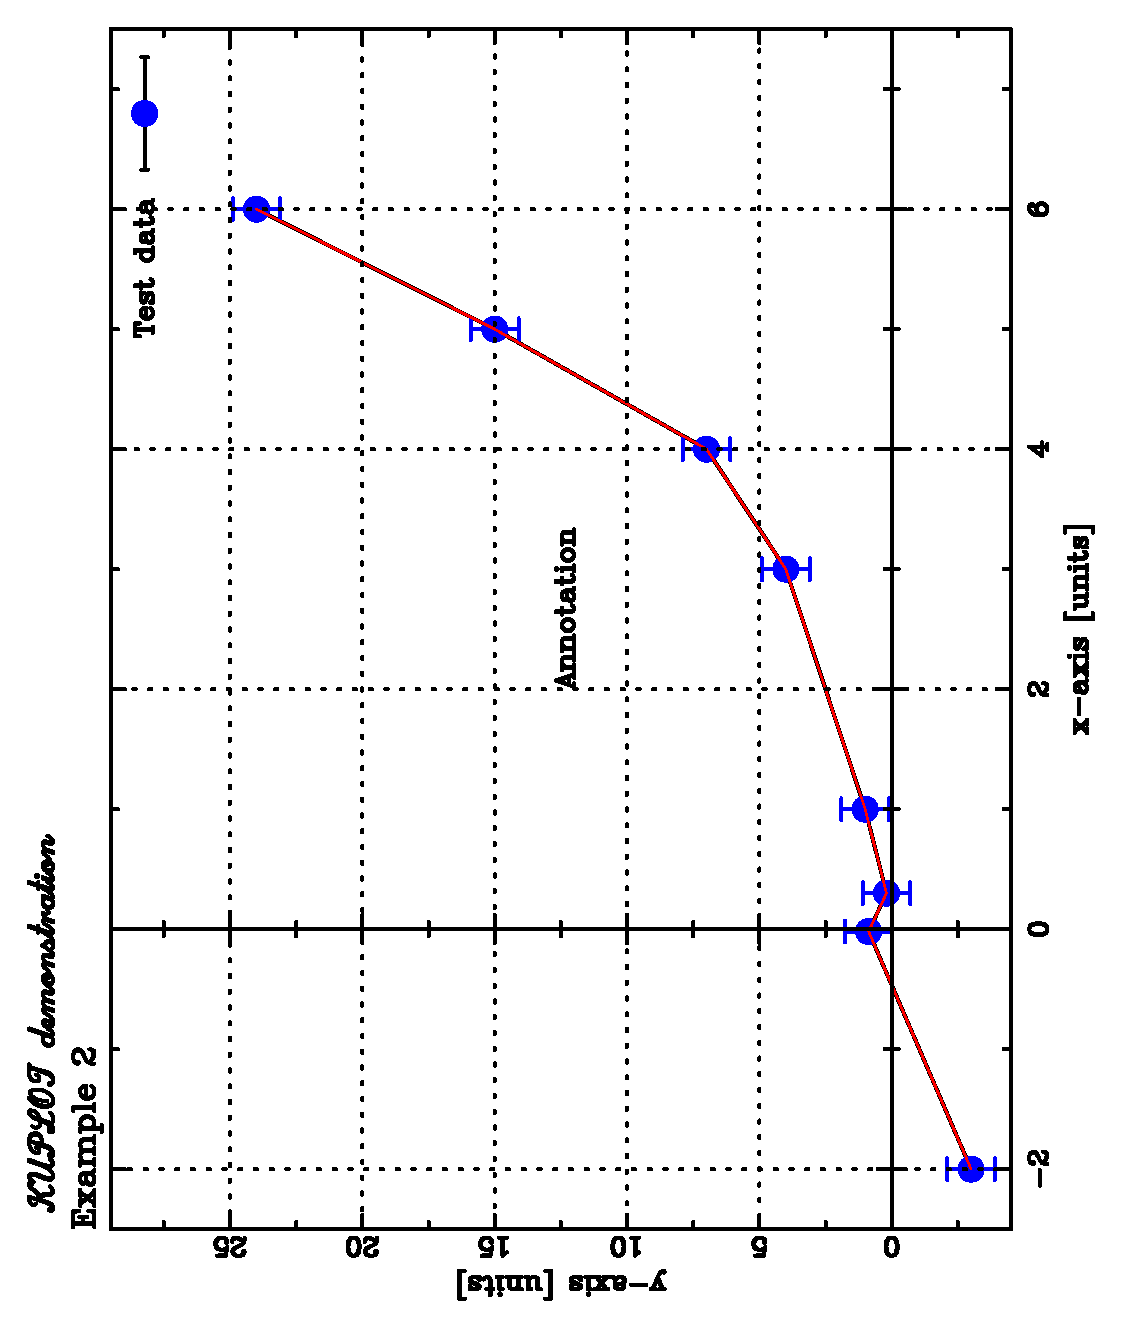
\includegraphics[width=3.0in, angle=270.0]{pl1.2.eps}
   \caption{Customized {\it KUPLOT} plot}
   \label{pl1-fig2}
\end{figure}

\section{Making a nicer plot \label{1d-change}}

In the example shown in Figure \ref{pl1-fig1} we have simply used
the defaults of {\it KUPLOT} and plotted the data set directly. The
program {\it KUPLOT} offers a variety of commands to alter the
appearance of the plot itself and the representation of each loaded
data set. We are using the same data set {\it test.xy} as in the
previous example (with added $\sigma$ values) and create the plot
shown in Figure \ref{pl1-fig2}. The macro file used to create this
plot is listed below. Note, that the line numbers are added for easy
reference within this manual and are not part of the actual macro
file.
%
\begin{MacVerbatim}
      1  load xy,test.xy
      2  #
      3  achx x-axis [units]
      4  achy y-axis [units]
      5  tit1 \fs KUPLOT demonstration
      6  tit2 Example 2
      7  #
      8  grid on
      9  fnam off
     10  #
     11  skal -2.5,7.5,-4.5,29.5
     12  mark 2,5
     13  #
     14  lcol 1,6
     15  lwid 1,0.5
     16  mtyp 1,3
     17  mcol 1,3
     18  msiz 1,0.4
     19  etyp 1,2
     20  #
     21  sleg 1,"Test data"
     22  sann 1,"Annotation",2,12
     23  plot
\end{MacVerbatim}
%
In line 1 of this macro we read the data set from file {\it test.xy}
as in the previous example.  The axes labels and the text for the
first and second title line are set in lines 3--6. The grid of
dashed lines at positions of the major tick marks is enabled in line
8 and the plotting of the filenames corresponding to the data sets
in the upper left corner of the plot is switched off (line 9). Next
we define the extend of the plot (line 11) to be from -2.5 to 7.5 in
the x-direction and from -4.5 to 29.5 in the y-direction. The tick
mark interval is set to 2.0 and 5.0 (line 12). All these settings
affected the complete plot, whereas the following commands act on
data set 1, which is given as the first parameter to all commands in
lines 14--19.  First the line color is set to black (line 14).  The
first six colors are coded as the 6 default pen colors on a HP
plotter, i.e.  red, green, blue, purple, yellow and black. Those
default colors can be redefined using the command {\tt color}.  In
the following lines, the line width, marker type, marker color and
marker size are defined (lines 16--18).  The different marker types
supported by {\it KUPLOT} are shown in Figure \ref{pl1-fig3}. In
addition to the markers shown, {\it KUPLOT} can access all markers
defined in the {\it PGPLOT} library. The marker number is simply 100
plus the {\it PGPLOT} marker code. Refer to the {\it PGPLOT}
documentation for a list of those markers. Error bars in y-direction
based on the $\sigma_{y}$ values read from the input file {\it
test.xy} are enabled in line 19. Marker types -1, -2 and -3 will
plot the $x$, $y$ or $x,y$ coordinated instead of a marker symbol.
The caption "Test data" is defined in line 21 and the annotation
"Annotation" at the coordinates (2.0,12.0) is specified by the {\tt
sann} command in line 22. Note, the value 1 in line 30 stands for
the first annotation and not for data set one. Finally the plot is
displayed on the screen (line 23).
%
\begin{figure}[!tb]
   \centering
   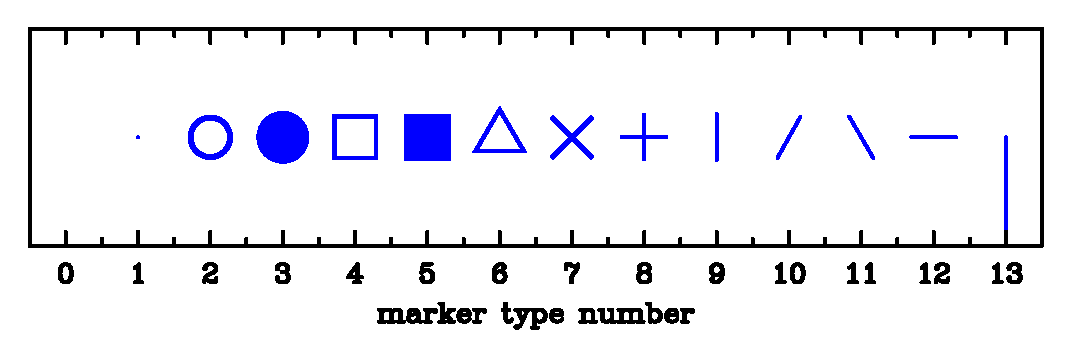
\includegraphics[scale=0.6]{pl1.3.eps}
   \caption{{\it KUPLOT} marker types}
   \label{pl1-fig3}
\end{figure}
%
\begin{figure}[!tb]
   \centering
   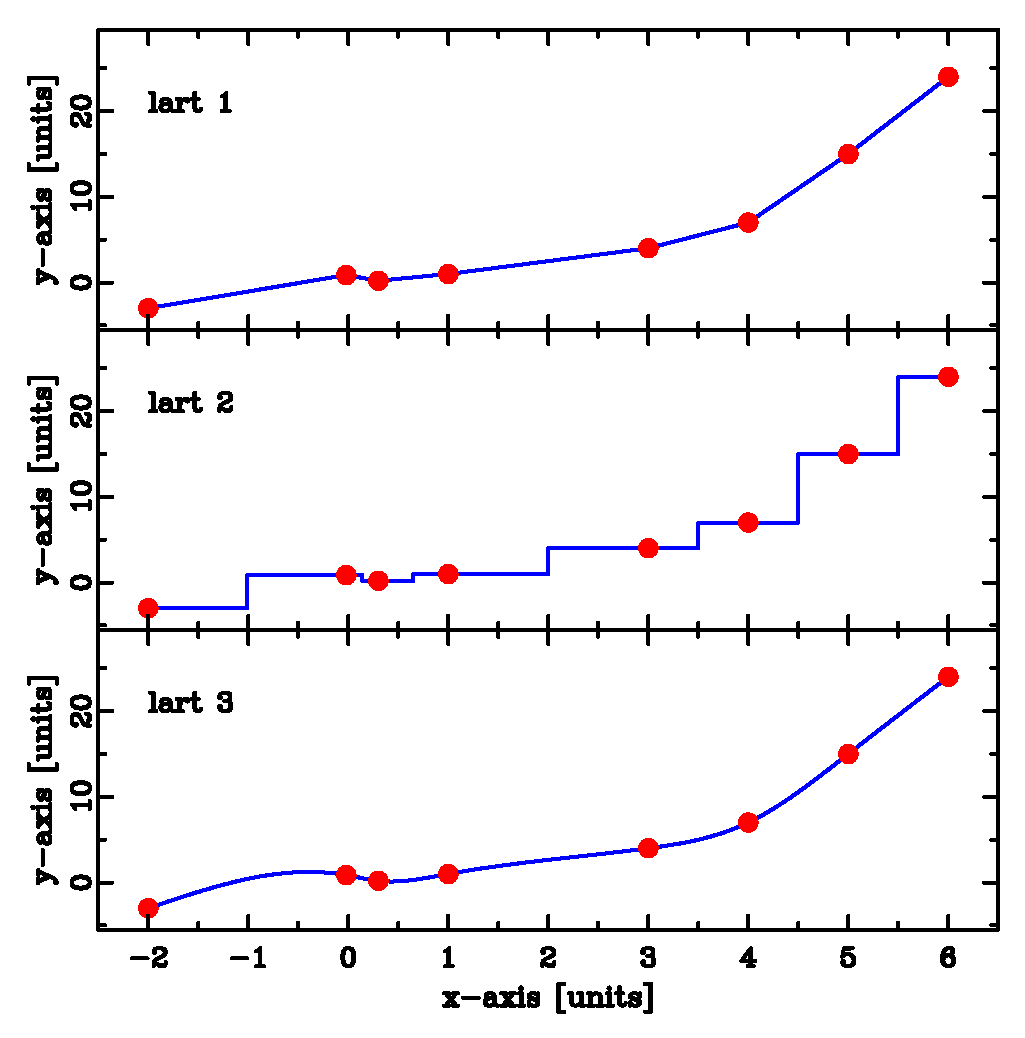
\includegraphics[scale=0.6]{pl1.4.eps}
   \caption{{\it KUPLOT} plotting styles}
   \label{pl1-fig4}
\end{figure}
%
In this example, the data points $(x_{i},y_{i})$ were simply
connected by a straight line.  {\it KUPLOT} offers two alternative
plotting styles: a histogram style and cubic spline interpolation.
The style is selected by the {\tt lart} command followed by the data
set number and the desired style. Style 1 is the default and
connects the data points by a straight line as in the previous
example ({\tt lart 1,1}).  This style is shown in Figure
\ref{pl1-fig4} in the bottom view graph.  The histogram style 2 is
shown in the middle view graph of the same Figure.  Here each data
point $(x_{i},y_{i})$ sits in the center of a histogram step. The
command to change the plotting style of data set 1 to histogram
would be {\tt lart 1,2}. The third mode ({\tt lart 1,3} for data set
1) is cubic spline interpolation. The interpolated spline goes
through all data points $(x_{i},y_{i})$ and has a continuous first
derivative. The spline interpolation of the data set {\it test.xy}
can be seen as top view graph in Figure \ref{pl1-fig4}. The default
number of interpolated points for a plot is 500. However, the value,
determined by the variable {\it MAXSP} might be altered in the file
{\it kuplot.inc} before {\it KUPLOT} is compiled.

%------------------------------------------------------------------------

\section{Fonts and special characters \label{1d-char}}

The program {\it KUPLOT} offers the user various ways to alter the
appearance of the text parts of the plot. All these functions are
accessed by the command {\tt font}. If no parameters are given, the
current settings will be displayed on the screen, as shown below:
%
\begin{table}[!bt]
\centering
\begin{tabularx}{\textwidth}{|c|X|}
  \hline
  {\bf Command} & {\bf Function} \\
  \hline\hline
   $\backslash$u  & start superscript, or end subscript \\
   $\backslash$d  & start sub-, or end superscript \\
   $\backslash$b  & backspace (draw next character on top of current one) \\
   $\backslash$fn & switch to normal font (1) \\
   $\backslash$fr & switch to roman font  (2) \\
   $\backslash$fi & switch to italic font (3) \\
   $\backslash$fs & switch to script font (4) \\
  \hline
   $\backslash\backslash$  & backslash  \\
   $\backslash$x  & multiplication sign $\times$ \\
   $\backslash$.  & centered dot $\cdot$ \\
   $\backslash$A  & \AA \\
  \hline
\end{tabularx}
\caption{\label{pl1-tab2}Text control characters}
\end{table}
%
\begin{MacVerbatim}
   Font settings for frame no.:   1
      Overall font scaling factor  :   2.50

      Font  where ?              size   fontname            font-id   color
      ---------------------------------------------------------------------
        1   Main title line       16.  Roman                    2       6
        2   Subtitle line         14.  Roman                    2       6
        3   Axis labels           12.  Roman                    2       6
        4   Numbers at axis       12.  Roman                    2       6
        5   Text in text frame    12.  Standard                 1       6
        6   Filename & caption    12.  Roman                    2       6
\end{MacVerbatim}
%
As can be seen from the output, there are six different types of
fonts, the main and second title line, the axis labels, the axis
numbering, text in a text frame (see section \ref{frame}) and
finally the font used for annotations and captions. Each of those
types is associated with a font size given in points, a font style
given as name (e.g. Roman) and number (e.g. 2) and finally a color
in our example pen number 6 or black. The four font styles
available in {\it KUPLOT} are shown in Figure \ref{pl1-fig5}. {\it
KUPLOT} allows the user to apply an overall scale factor to the
font size or change font sizes individually. As an example let us
change the color of the first title line to red. This would be
done using the command:
%
\begin{MacVerbatim}
    font col,1,1
\end{MacVerbatim}
%
The first parameter tells {\it KUPLOT} what we want to change,
here the color. Next we have the number of the font type, here 1
for the first title line. Finally we specify the desired color,
here pen 1 for red. One benefit of using the {\it PGPLOT} library
is that the user can access special characters and commands within
all text lines, e.g. titles, axis labels and text in text frames.
The supported control commands are listed in Table \ref{pl1-tab2}
and a list of Greek characters is given in Table \ref{pl1-tab3}.
For example to create an axis label \AA$^{-2}$ the text input
would read {\it $\backslash$A$\backslash$u-2$\backslash$d}. Note
that sub- and superscript always have to be given in pairs.
%
\begin{table}[!tbp]
\centering
\begin{tabular}{|c|cc|cc||c|cc|cc|}
  \hline
   alpha   & $\backslash$ga  & $\alpha$   & $\backslash$gA &   $A$        &
   beta    & $\backslash$gb  & $\beta $   & $\backslash$gB &   $B$        \\
   gamma   & $\backslash$gg  & $\gamma$   & $\backslash$gG &   $\Gamma$   &
   delta   & $\backslash$gd  & $\delta$   & $\backslash$gD &   $\Delta$   \\
   epsilon & $\backslash$ge  & $\epsilon$ & $\backslash$gE &   $E$        &
   zeta    & $\backslash$gz  & $\zeta $   & $\backslash$gZ &   $Z$        \\
   theta   & $\backslash$gh  & $\theta$   & $\backslash$gH &   $\Theta$   &
   iota    & $\backslash$gi  & $\iota $   & $\backslash$gI &   $I$        \\
   kappa   & $\backslash$gk  & $\kappa$   & $\backslash$gK &   $K$        &
   lambda  & $\backslash$gl  & $\lambda$  & $\backslash$gL &   $\Lambda$  \\
   mu      & $\backslash$gm  & $\mu   $   & $\backslash$gM &   $M$        &
   nu      & $\backslash$gn  & $\nu   $   & $\backslash$gN &   $N$        \\
   xi      & $\backslash$gc  & $\xi   $   & $\backslash$gC &   $\Xi   $   &
   omicron & $\backslash$go  & $o     $   & $\backslash$gO &   $O     $   \\
   pi      & $\backslash$gp  & $\pi   $   & $\backslash$gP &   $\Pi   $   &
   rho     & $\backslash$gr  & $\rho  $   & $\backslash$gR &   $P     $   \\
   sigma   & $\backslash$gs  & $\sigma$   & $\backslash$gS &   $\Sigma$   &
   tau     & $\backslash$gt  & $\tau  $   & $\backslash$gT &   $T     $   \\
   upsilon & $\backslash$gu  & $\upsilon$ & $\backslash$gU &   $\Upsilon$ &
   phi     & $\backslash$gf  & $\phi  $   & $\backslash$gF &   $\Phi  $   \\
   chi     & $\backslash$gx  & $\chi  $   & $\backslash$gX &   $X     $   &
   psi     & $\backslash$gq  & $\psi  $   & $\backslash$gQ &   $\Psi  $   \\
   omega   & $\backslash$gw  & $\omega$   & $\backslash$gO &   $\Omega$   &
           &                 &            &                &              \\
  \hline
\end{tabular}
\caption{\label{pl1-tab3}Access to Greek characters}
\end{table}
%
These examples can only give a brief introduction in the different
commands of {\it KUPLOT} allowing the user to alter the appearance
of the plot. For details on these commands and their parameters
refer to the online help, the command reference or the interactive
tutorial.
%
\begin{figure}[!tb]
   \centering
   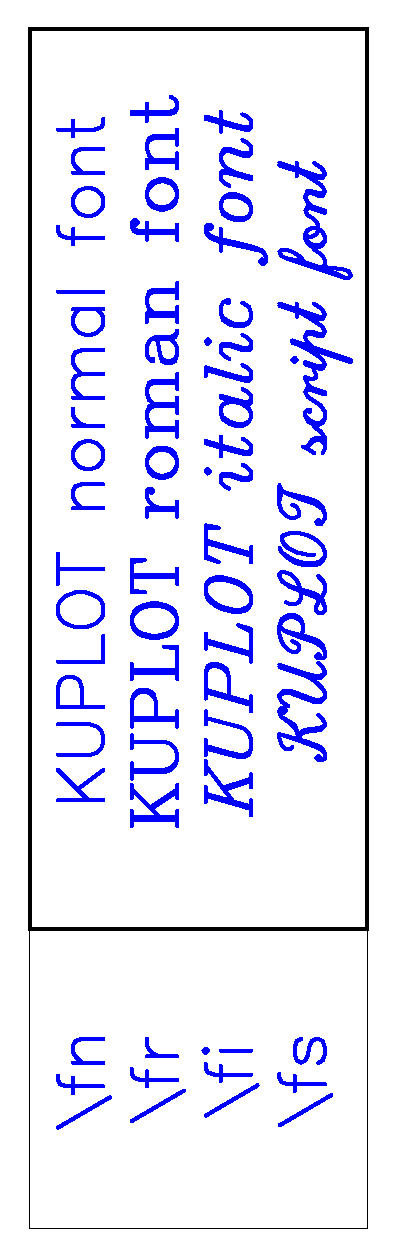
\includegraphics[scale=0.5, angle=270.0]{pl1.5.eps}
   \caption{{\it KUPLOT} fonts}
   \label{pl1-fig5}
\end{figure}

%------------------------------------------------------------------------

\section{Drawing bonds \label{1d-bond}}

The program {\it KUPLOT} allows the user to connect points in the
plot that are separated by a given distance. The distance is
specified relative to the current x-axis. To calculate the
distances, the aspect ratio and the angle between the axes is used.
These values can be defined by the user via the commands {\tt aver}
and {\tt angl} as we will discuss in somewhat more detail in section
\ref{2d-change}. Consequently you will get the desired connection
only for the correct aspect ratio and angle between the axes. This
feature can be used to include bonds when plotting a structure file
exported by {\it DISCUS}. An example for the compound PHTP
(Perhydrotriphenylen) is shown in Figure \ref{pl1-fig6}. The macro
file used to create this picture is listed below:
%
\begin{MacVerbatim}
      1  rese
      2  load cr,phtp.cr
      3  #
      4  skal 0.0,28.8,0.0,28.8
      5  mark 14.4,14.4
      6  #
      7  aver 1.0
      8  angl 120.0
      9  #
     10  msiz 1,0.35
     11  grid on
     12  fnam off
     13  #
     14  achx a-axis (\A)
     15  achy b-axis (\A)
     16  #
     17  bond 1,1.4,0.2,1,1,1.5
     18  #
     19  plot
\end{MacVerbatim}
%
First we reset the program and read the data (line 2). In line 4 the
plot area is defined followed by the setting for the tick mark
interval (line 5). In our case the lattice parameter is
$a=b=14.4$\AA. The command {\tt aver} defines the ratio between
units on the y- and x-axis. Since both are in \AA, the desired ratio
is one. The angle between the axes is set to 120$^{\circ}$ (line 8).
Next we set the marker size (line 10), turn the plotting of the grid
on (line 11) and disable the plotting of the filenames (line 12).
The axes labels are set in lines 14 and 15. So far nothing new, now
comes the command {\tt bond} that defines the bonds between carbon
atoms we like to plot. The first parameter 1 is the number of the
bond definition. {\it KUPLOT} allows one to define multiple
distances. The second and third parameter set the distance to
$1.4$\AA\ $\pm 20$\%. The last optional parameters in line 17 set
the bond color to red (pen 1), select a solid line (type 1) and set
the line width to $1.5$. All that remains is to plot the result
(line 19). One should be aware that {\it KUPLOT} calculates the
distances between {\it all} data points and compares the to the
selected distance interval which can be rather slow for large data
file. To disable a bond definition simply reenter the command with
distance zero, e.g. {\tt bond 1,0.0}.
%
\begin{figure}[!tb]
   \centering
   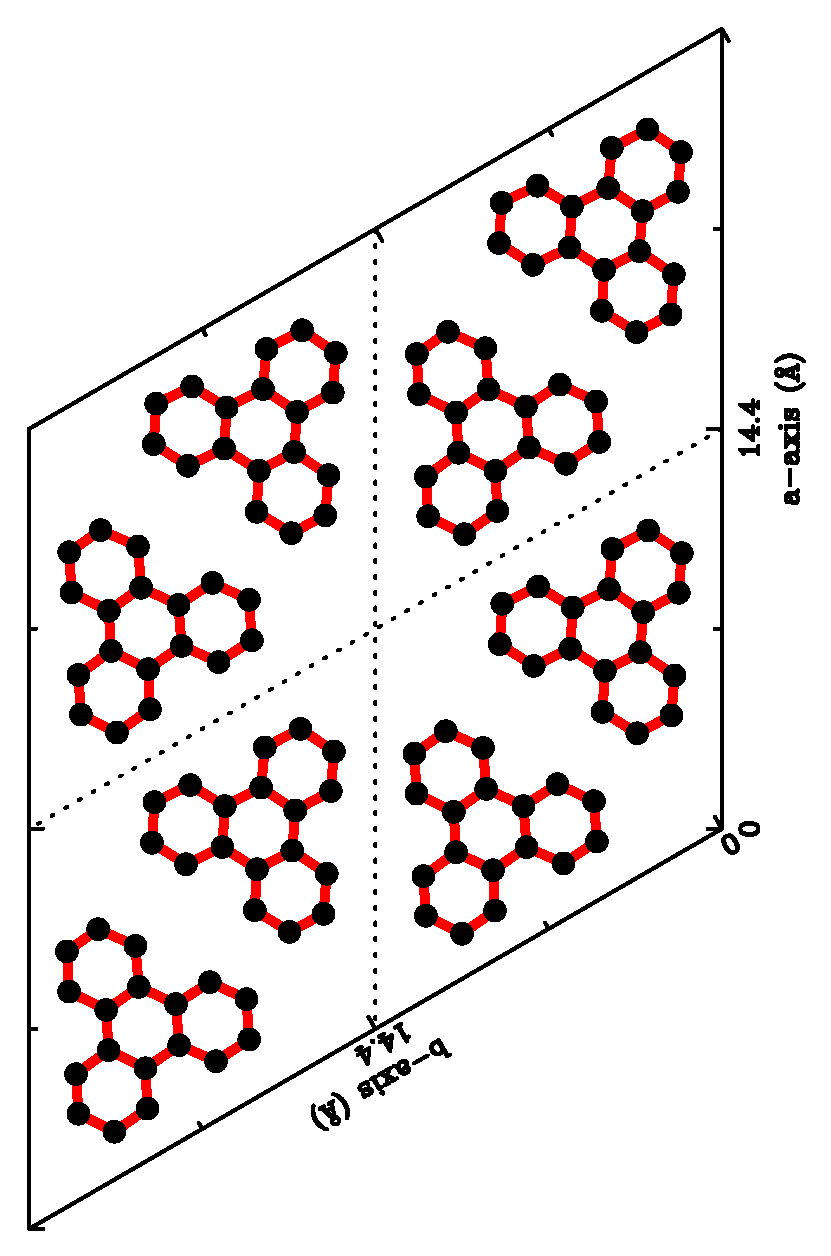
\includegraphics[scale=0.5, angle=270.0]{pl1.6.eps}
   \caption{Example for plotting bonds}
   \label{pl1-fig6}
\end{figure}

%------------------------------------------------------------------------

\section{Filling of areas\label{1d-fill}}

Sometimes to enhance the visibility of plot, it is desired to fill
the area under a data set. A plot taken from our recent book {\it
Diffuse scattering and defect structure simulations - A cook book
using the program DISCUS} published by Oxford University Press is
shown in Figure \ref{pl1-fig6b}.
%
\begin{figure}[!tb]
   \centering
   \includegraphics[scale=0.5, angle=0.0]{pl1.6b.eps}
   \caption{Example for filling areas}
   \label{pl1-fig6b}
\end{figure}

The part setting the colors and filling options of the macro file
used to create the plot is shown here.

\begin{MacVerbatim}
   color 1,0.8,0.8,0.8
   color 2,0.6,0.6,0.6
   color 3,0.4,0.4,0.4
   #
   fill 1,3,5
   fill 2,2,5
   fill 3,1,5
\end{MacVerbatim}
%
The command {\tt color} sets the color for the different 'pens' of
{\it KUPLOT}. In this case colors one through three are assigned
three different shades of grey. The color is specified as red,
green, blue raging from 0 to 1. The command {\tt fill ik,c,t} then
selects filling for data set {\tt ik} using color or pen {\tt c} and
setting the fill style to {\tt f}. In our case style five
corresponds to a solid fill with a black border. Type {\tt help
fill} for a list of all fill styles.

%------------------------------------------------------------------------

\section{Saving data sets \label{1d-save}}

The program {\it KUPLOT} allows the user to save loaded data sets to
a file.  This might be necessary after a data set was altered or in
cases where only part of the data shall be saved.  To save a data
set, use the command {\tt ksav} followed by the number of the data
set to be saved.  After entering the {\tt ksav} sublevel, you need
to specify the output filename and the file format for the output
file. In this section we will only discuss the saving of 1D data
sets and the only available file format is {\tt xy} (see previous
example).  The following commands will save the loaded data set 1
(e.g.  {\it test.xy} from the example above):
%
\begin{MacVerbatim}
     1  ksav 1
     2    outfile export.xy
     3    form xy,0.0,5.0
     4    show
     5  run
\end{MacVerbatim}
%
In line 1 we enter the {\tt ksav} sublevel.  The parameter specifies
the data set we want to save, here data set 1.  Next the output
filename is set to {\it export.xy} (line 2).  The file format is set
to {\tt xy} and the optional further parameters give x-limits (line
3), i.e.  only data points with x-values between 0.0 and 5.0 will be
saved.  Note, that the default range are defined by the current plot
window limits.  Thus if the plot window set by the command {\tt
skal} is smaller than the extend of the actual data set, only point
that are visible in the current plot are saved if no limits are
given with the {\tt form} command.  The command {\tt show} (line 4)
lists the current limits and finally the data are written to the
specified file via the {\tt run} command (line 5).  The command {\tt
run} also exits the {\tt ksav} sublevel.  To exit without actually
writing a file use the {\tt exit} command.  \par

The {\tt ksav} command has many additional options to save 2D data
such as format conversion and the export of cross sections. These
functions are discussed in chapter \ref{2d-save}.

%------------------------------------------------------------------------

\section{Printing and exporting the plot \label{1d-print}}

Viewing the plot on the screen is one thing, but we certainly need
to print plot at some stage or save is for e.g. import in a text
processing program. {\it KUPLOT} supports two different output
formats that can be saved or used for printing. The defaults are
POSTSCRIPT and GIF associated with the parameters {\tt ps} and {\tt
pic} respectively. However, they can be set to any device supported
by {\it PGPLOT} by altering the variables {\it dev\_name} in the
file {\it blk\_appl.f} of the {\it KUPLOT} distribution. The
variable {\it dev\_prn} in the same file sets the default print
command. To print the current plot to the default printer, use {\tt
prin ps}. To reach other printers, the corresponding print command
can be specified as a second parameter to the {\tt prin} command as
in the example below:
%
\begin{MacVerbatim}
     prin ps,"lp -d myprinter -h "
\end{MacVerbatim}
%
Here the printer {\tt myprinter} is used. Check local documentation
or ask your system administrator how to access the desired printer.
In order to save the graphics file rather than printing it, use the
{\tt save} command with the first parameter being {\tt ps} or {\tt
pic} for POSTSCRIPT or GIF output respectively.  The second
parameter is the name of the output file, e.g. {\tt save
ps,plot.ps}.

%------------------------------------------------------------------------
